\chapter{Anexos}
\label{chap:anexos}

\section{Código en Julia del Mapa CL-CDMX}}

\lstinputlisting[language=Julia]{CodigoMuestra.jl}

\section{Tendencias de radiancia en las alcaldías de la Ciudad de México}}

\begin{figure}[H]
  \centering
    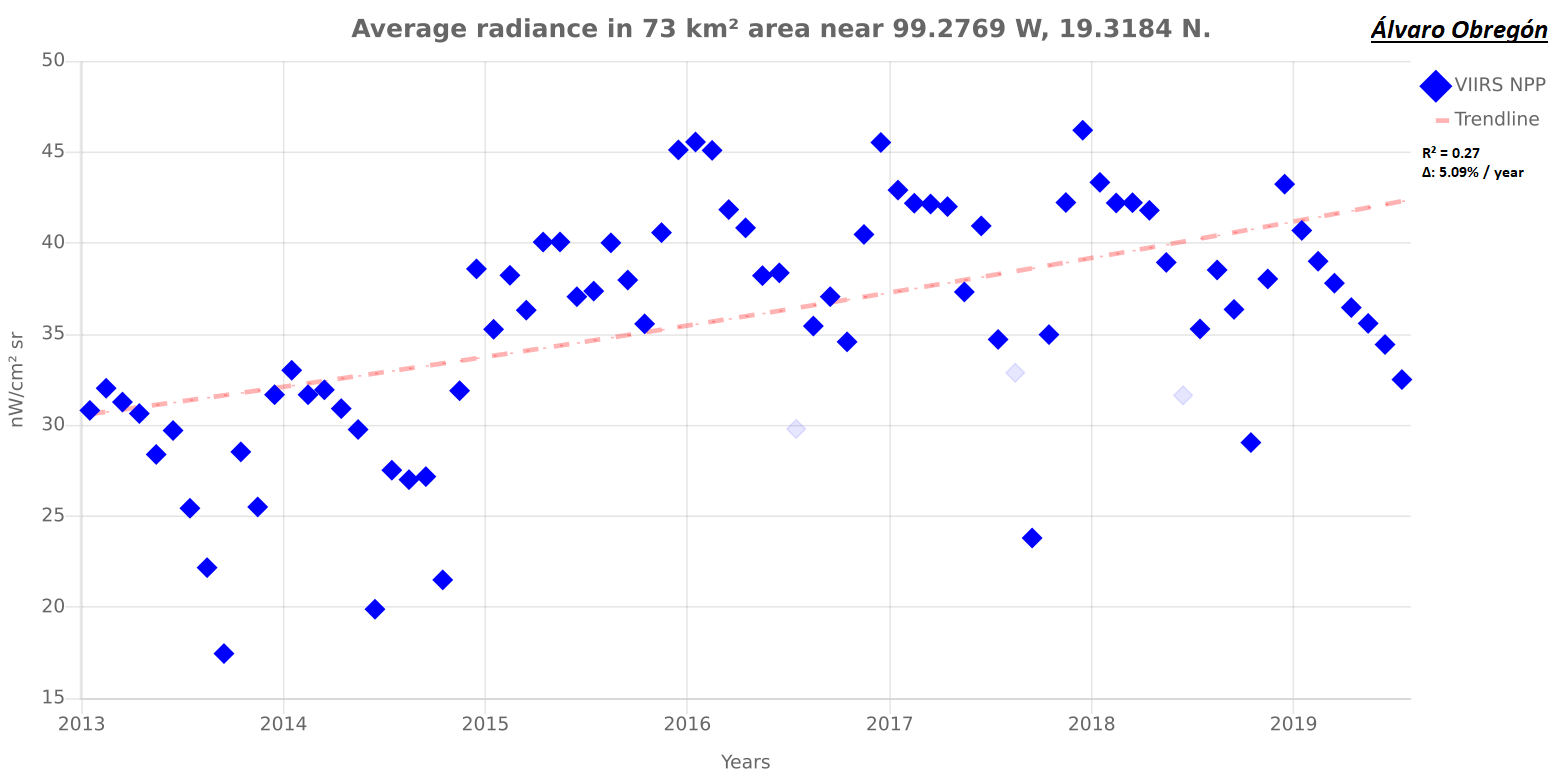
\includegraphics[width=1\textwidth]{AO}
  \caption{Tendencia de radiancia promedio para la alcaldía Álvaro Obregón}
  \label{radiancetrendsao}
\vspace{20mm} 
    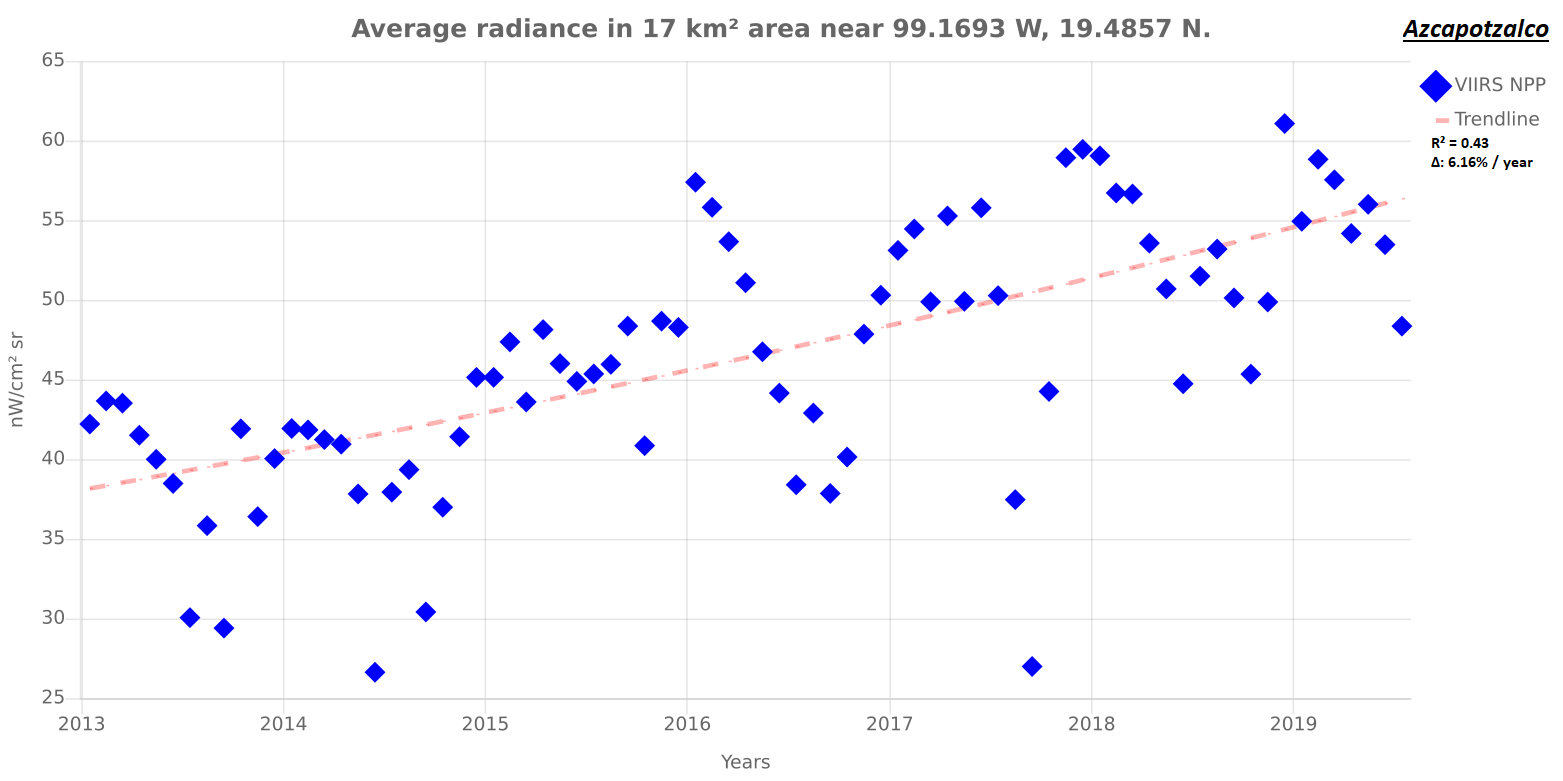
\includegraphics[width=1\textwidth]{AZ}
  \caption{Tendencia de radiancia promedio para la alcaldía Azcapotzalco}
  \label{radiancetrendsaz}
\end{figure}
\blindtext

\newpage

\begin{figure}[H]
  \centering
    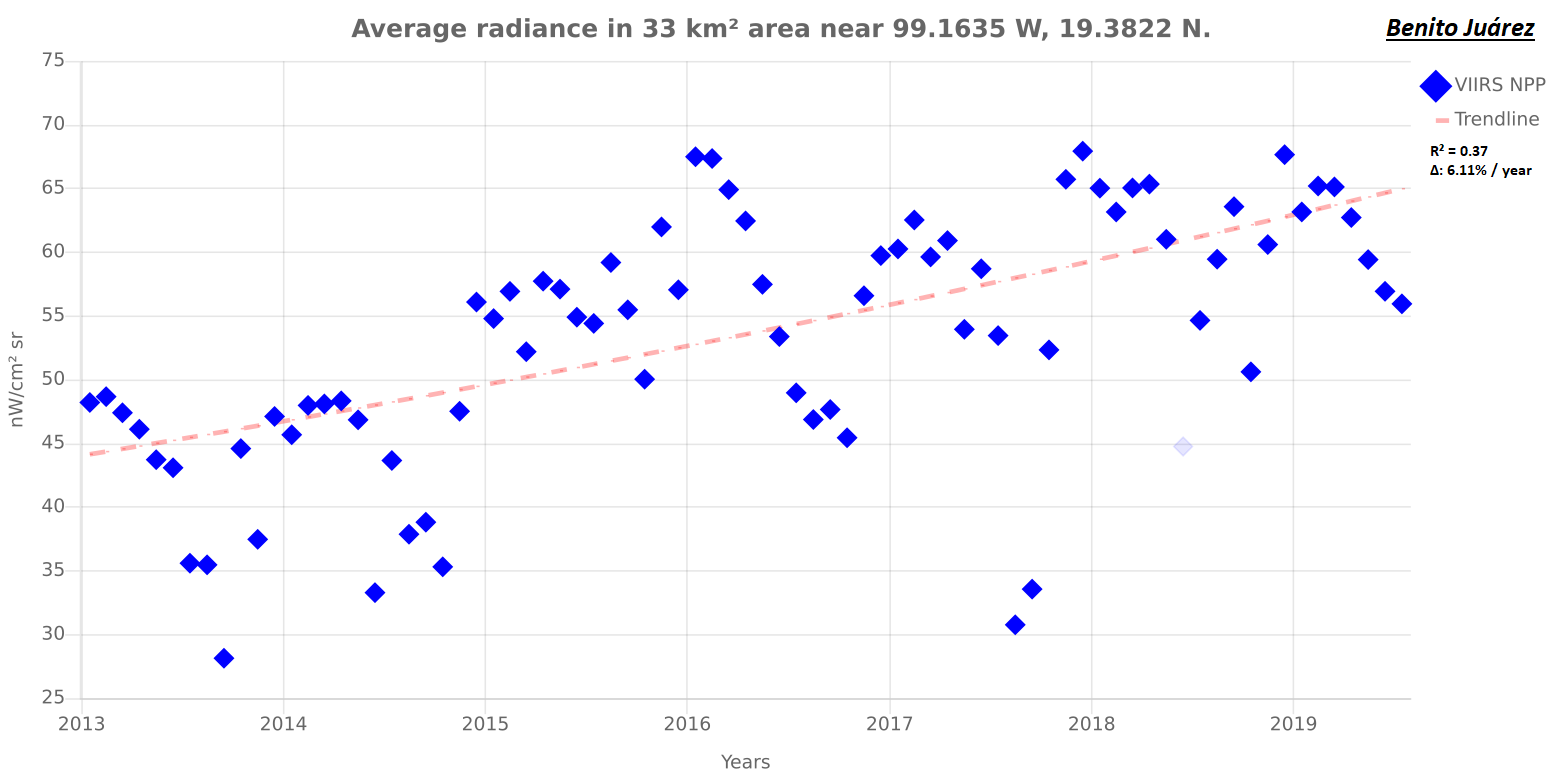
\includegraphics[width=1\textwidth]{BJ}
  \caption{Tendencia de radiancia promedio para la alcaldía Benito Juárez}
  \label{radiancetrendsbj}
\vspace{20mm} 
    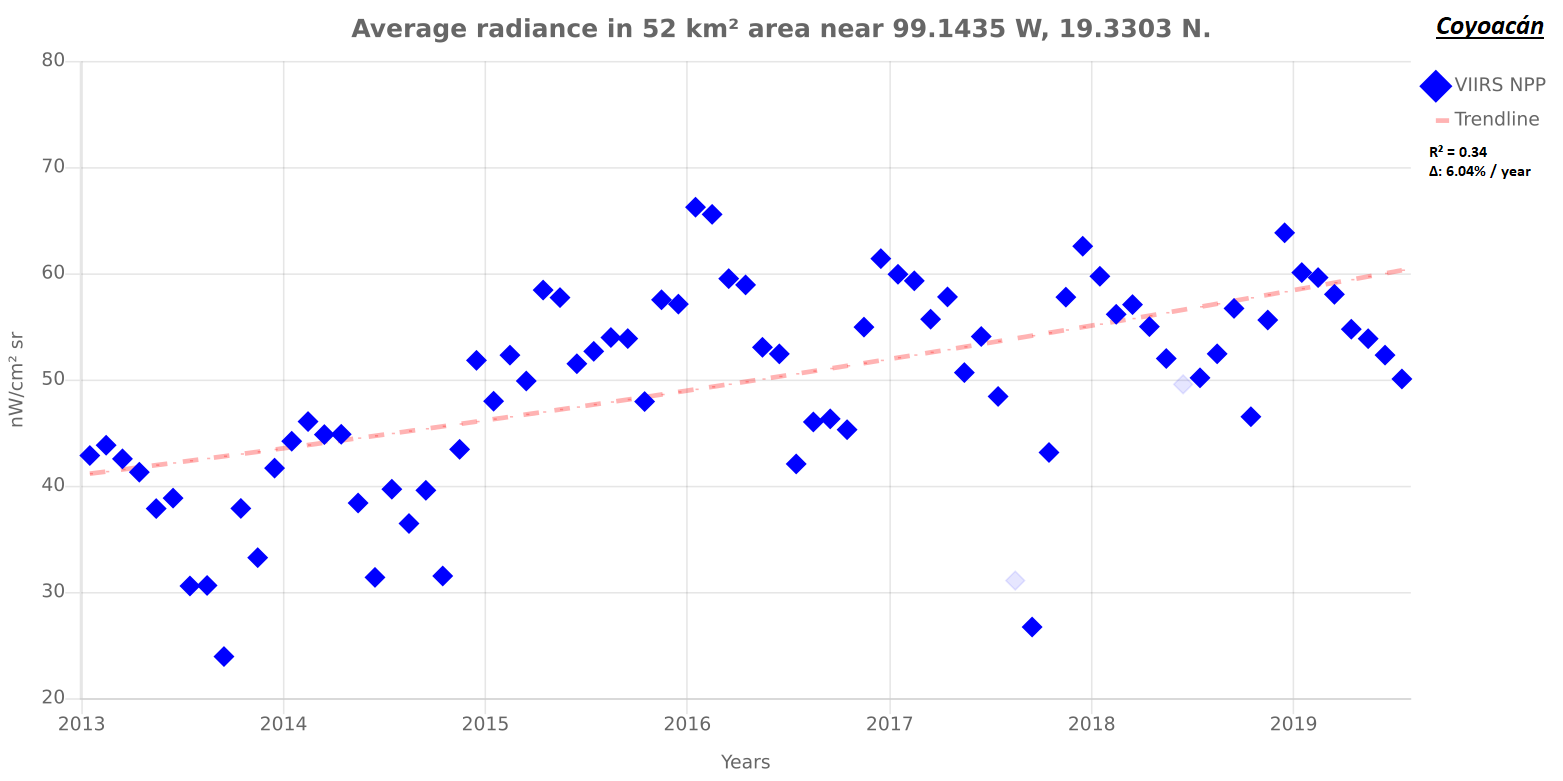
\includegraphics[width=1\textwidth]{CO}
  \caption{Tendencia de radiancia promedio para la alcaldía Coyoacán}
  \label{radiancetrendsco}
\end{figure}
\blindtext

\newpage

\begin{figure}[H]
  \centering
    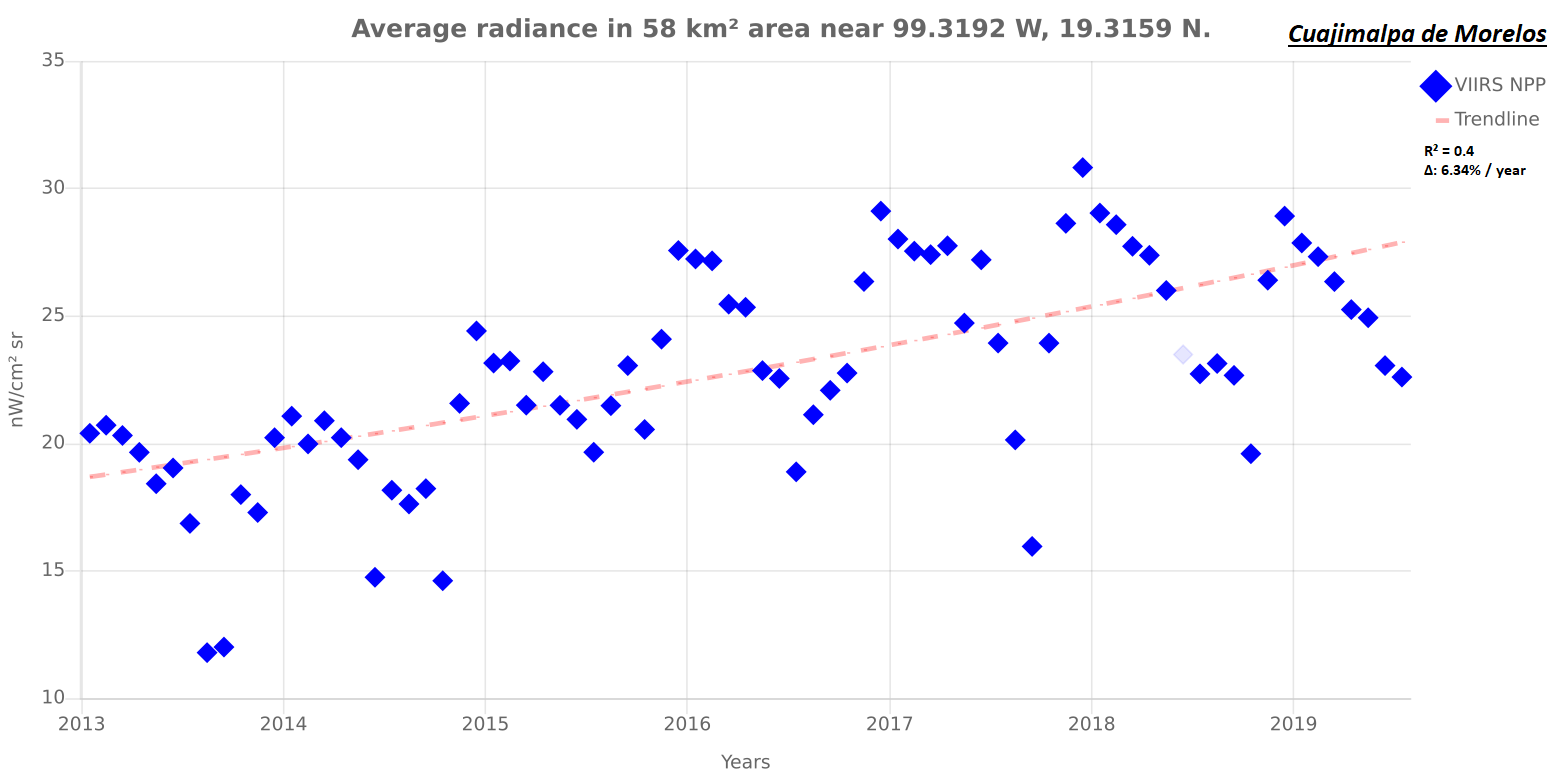
\includegraphics[width=1\textwidth]{CM}
  \caption{Tendencia de radiancia promedio para la alcaldía Cuajimalpa de Morelos}
  \label{radiancetrendscm}
\vspace{20mm} 
    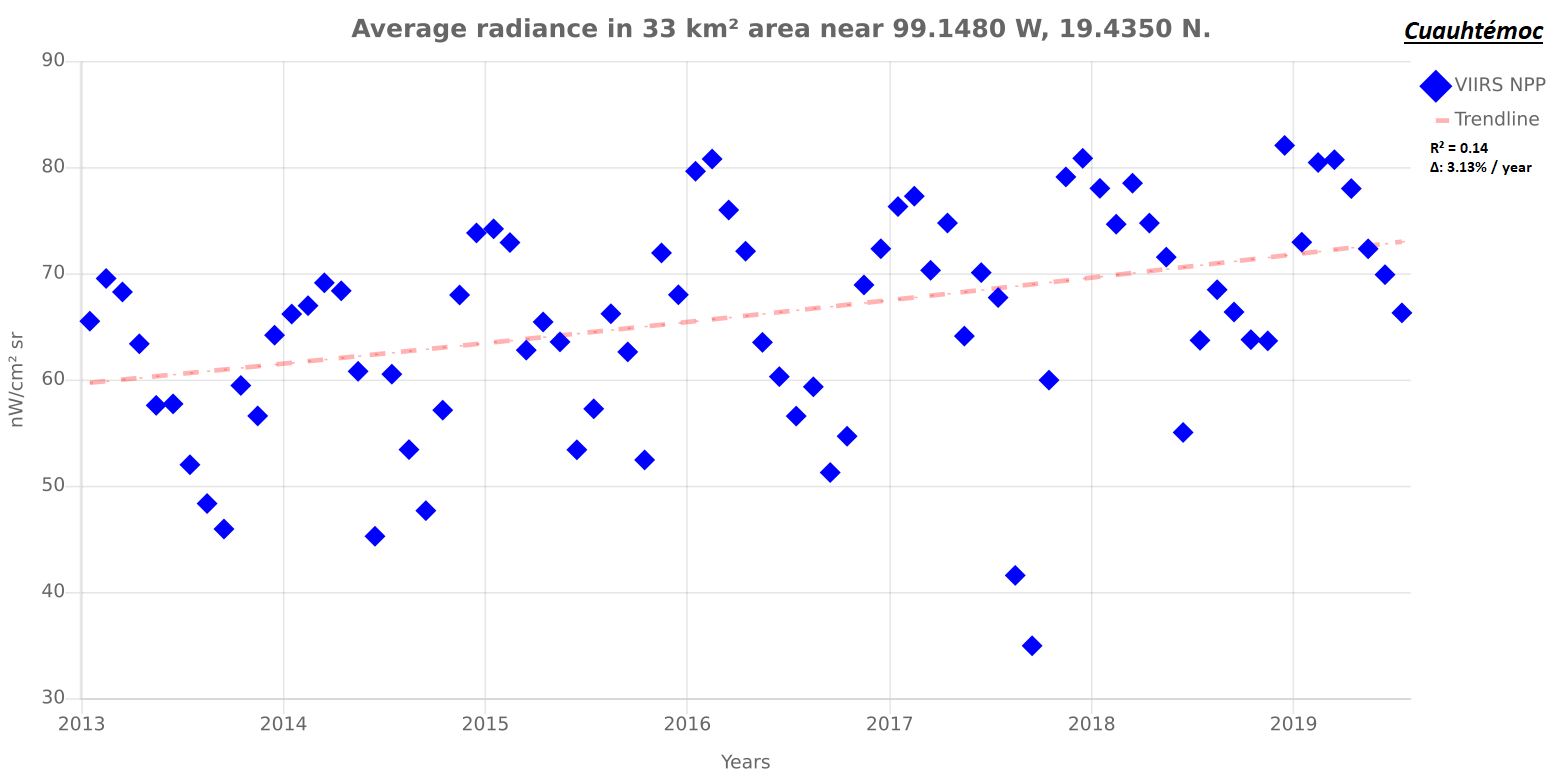
\includegraphics[width=1\textwidth]{CUA}
  \caption{Tendencia de radiancia promedio para la alcaldía Cuauhtémoc}
  \label{radiancetrendscua}
\end{figure}
\blindtext

\newpage

\begin{figure}[H]
  \centering
    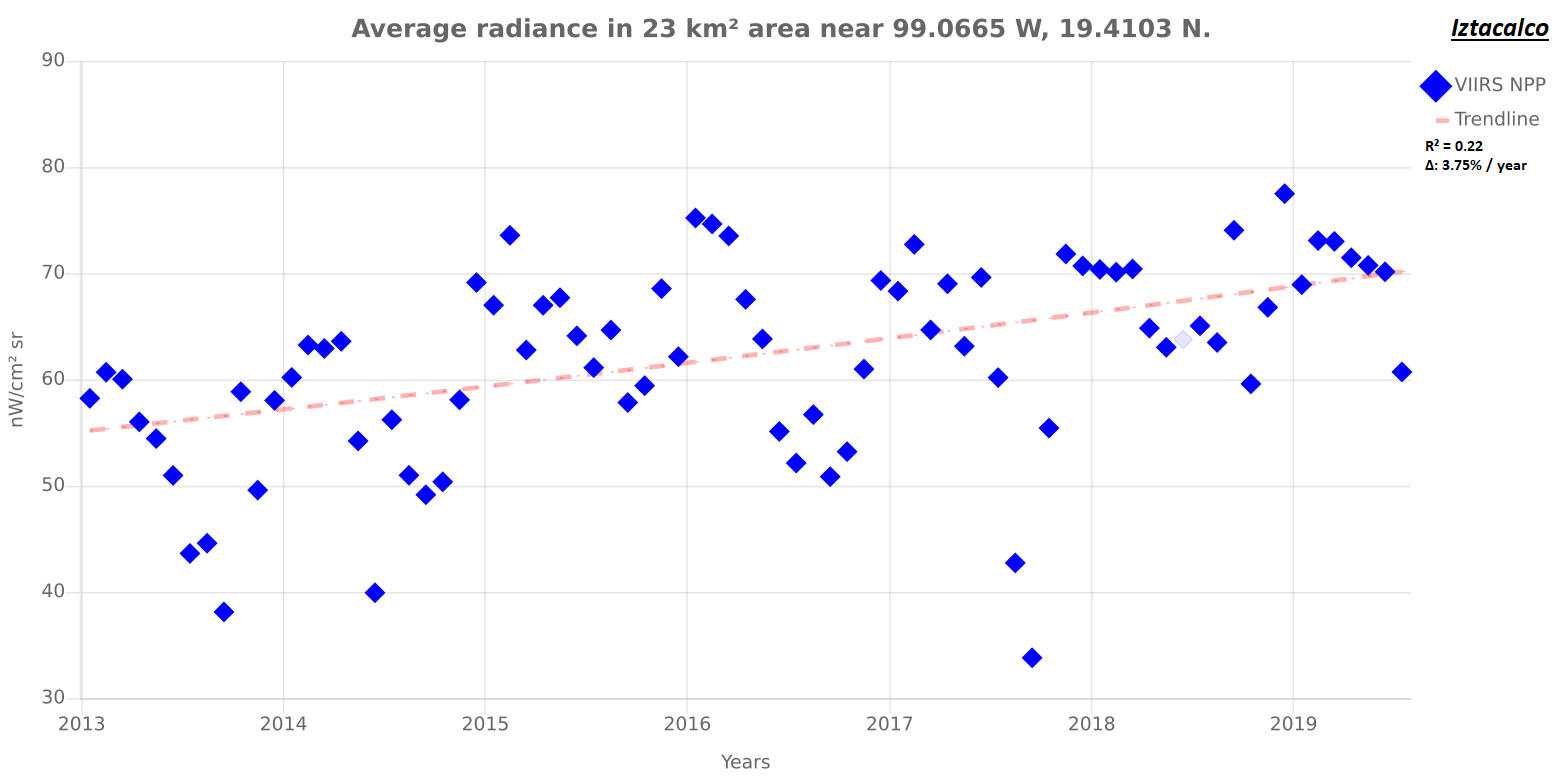
\includegraphics[width=1\textwidth]{IZT}
  \caption{Tendencia de radiancia promedio para la alcaldía Iztacalco}
  \label{radiancetrendsizt}
\vspace{20mm} 
    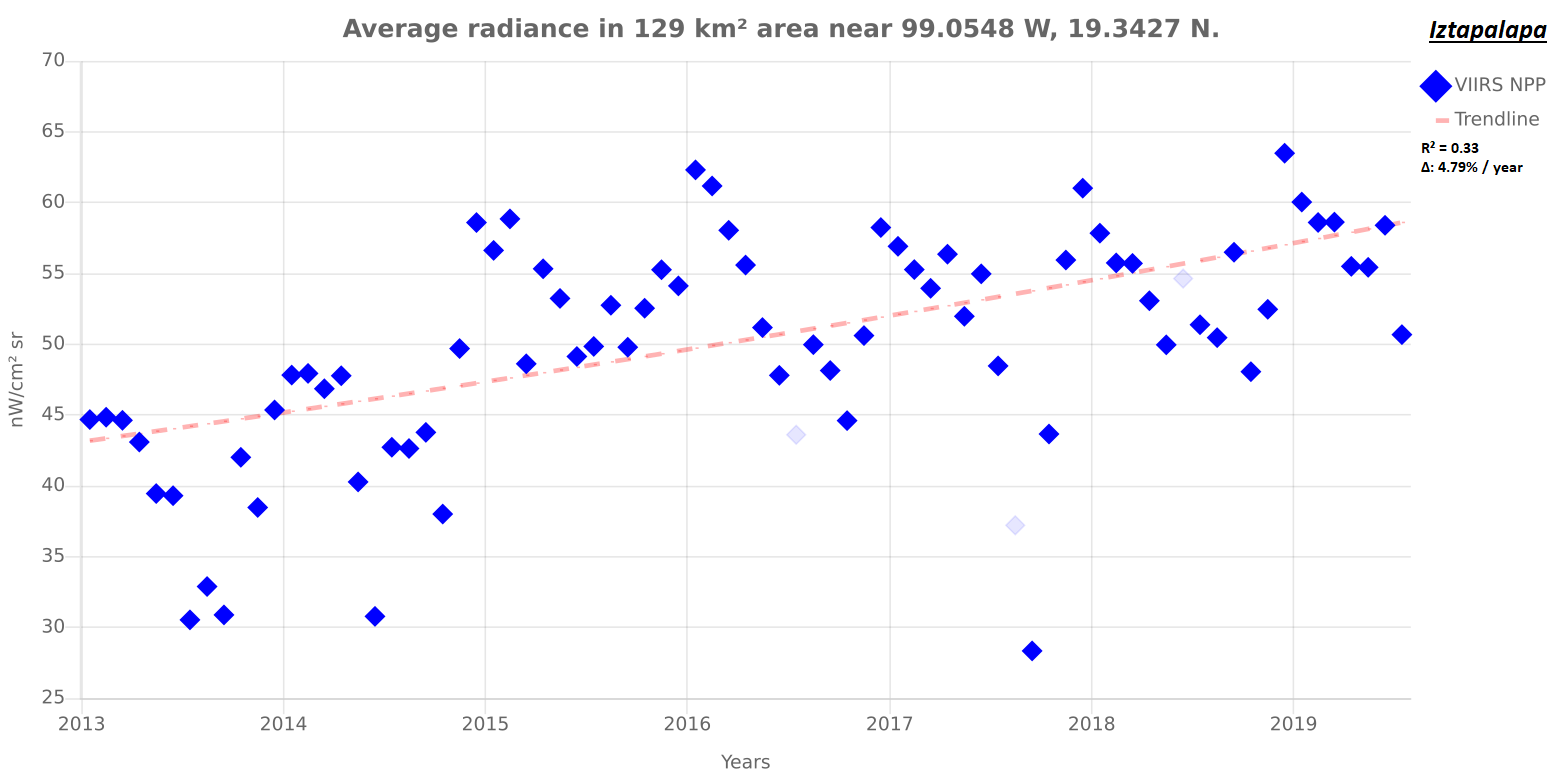
\includegraphics[width=1\textwidth]{IZP}
  \caption{Tendencia de radiancia promedio para la alcaldía Iztapalapa}
  \label{radiancetrendsizp}
\end{figure}
\blindtext

\newpage

\begin{figure}[H]
  \centering
    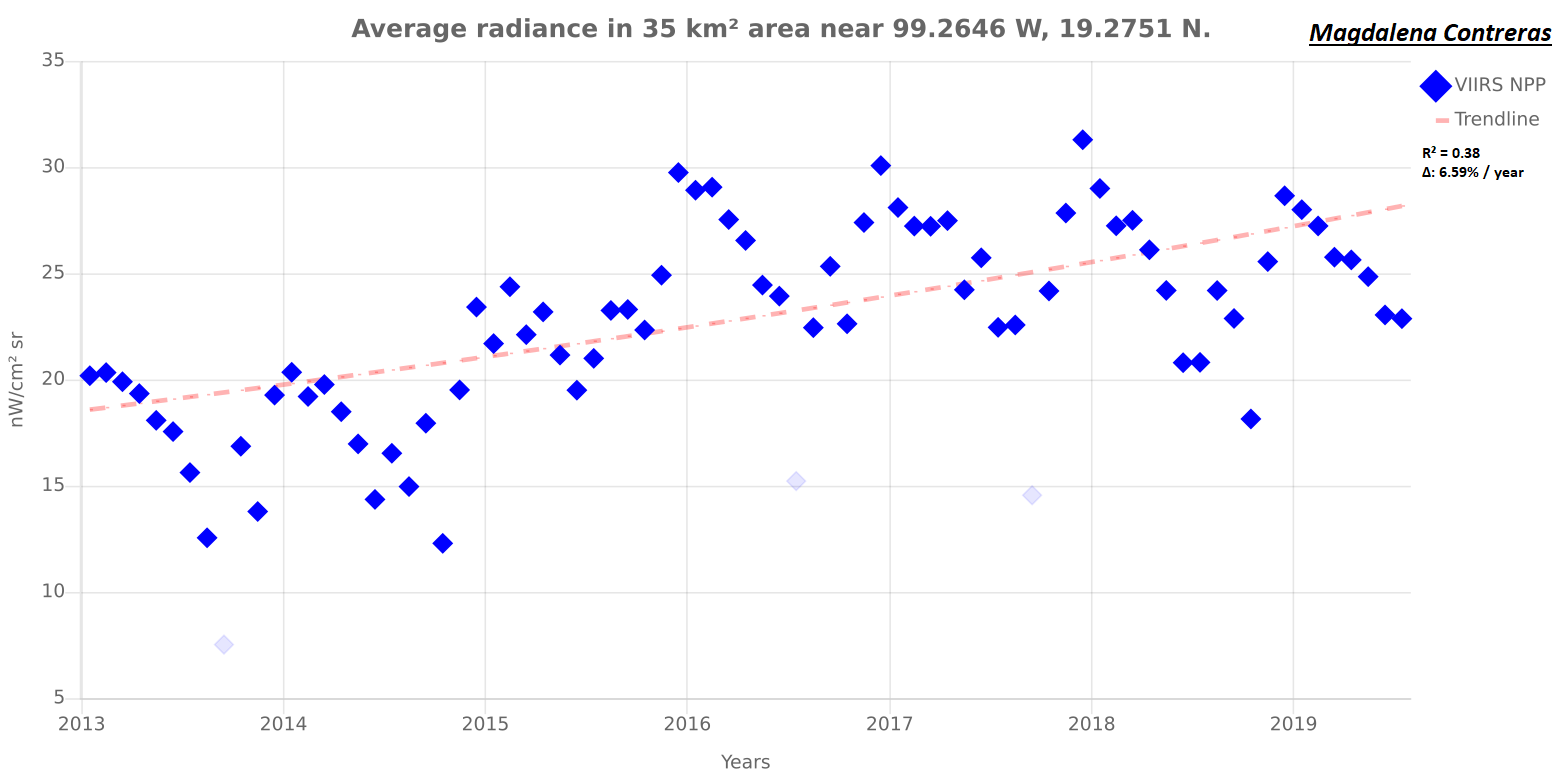
\includegraphics[width=1\textwidth]{MC}
  \caption{Tendencia de radiancia promedio para la alcaldía Magdalena Contreras}
  \label{radiancetrendsmc}
\vspace{20mm} 
    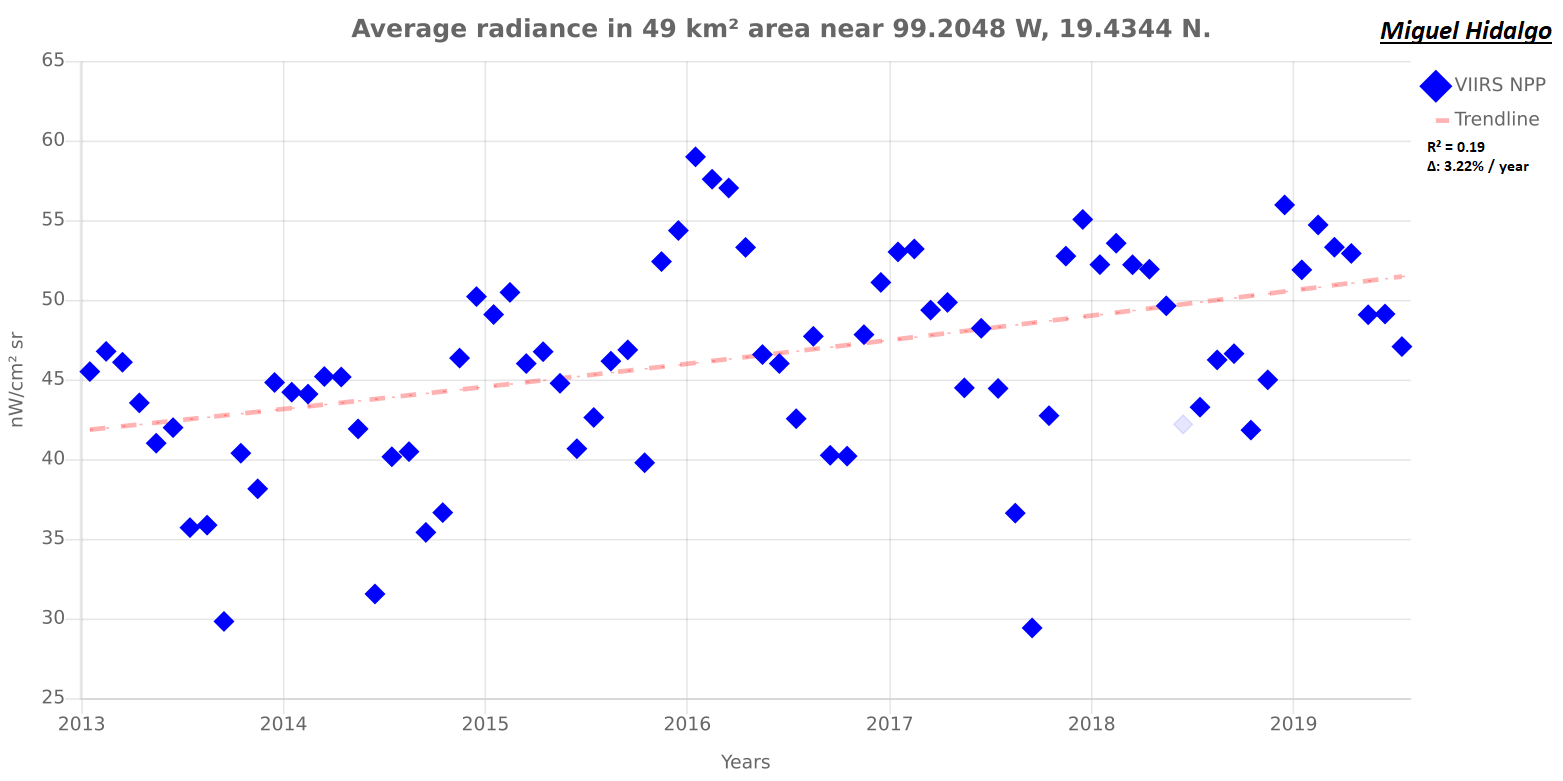
\includegraphics[width=1\textwidth]{MH}
  \caption{Tendencia de radiancia promedio para la alcaldía Miguel Hidalgo}
  \label{radiancetrendsmh}
\end{figure}
\blindtext

\

\begin{figure}[H]
  \centering
    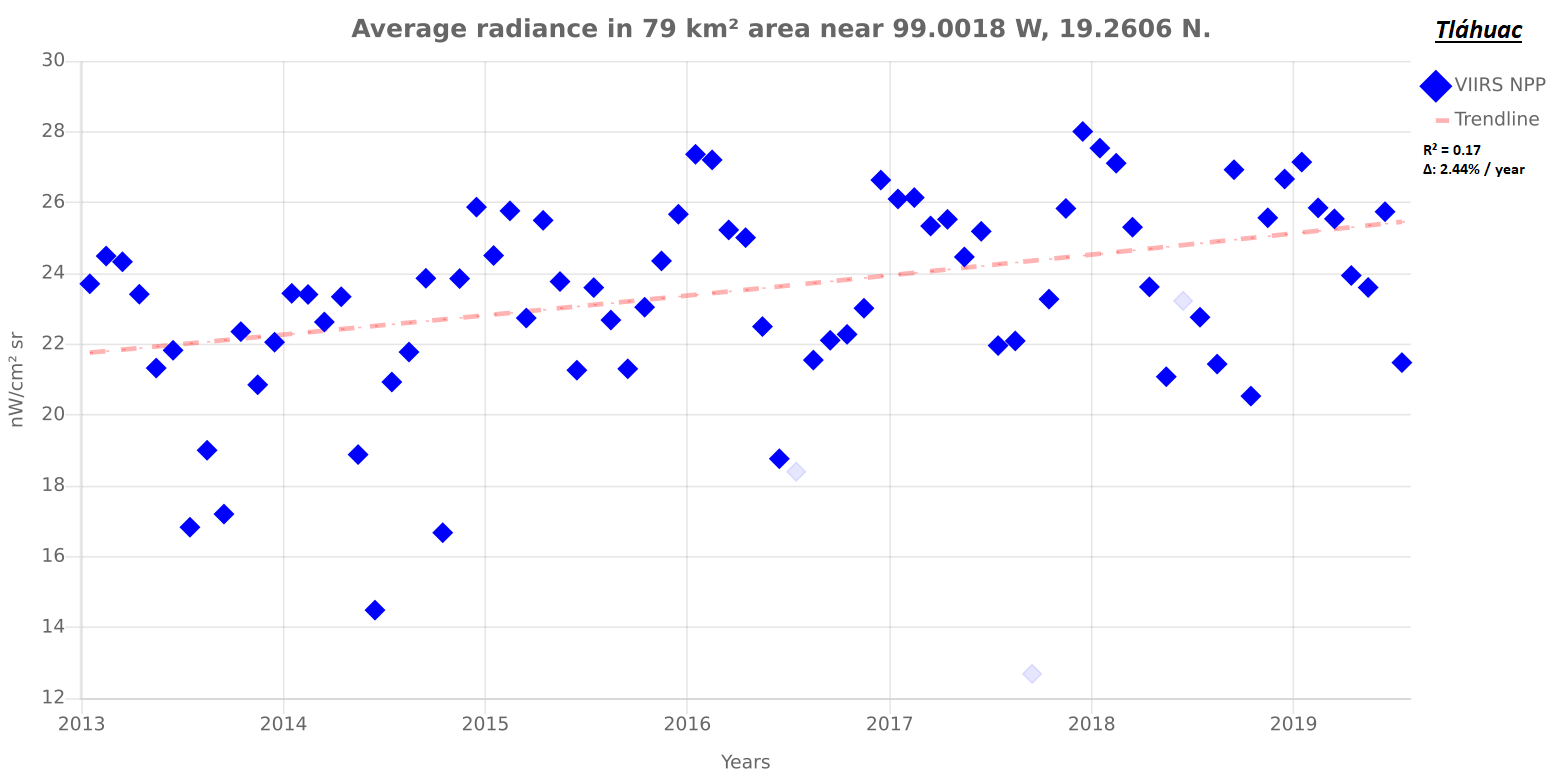
\includegraphics[width=1\textwidth]{TLAH}
  \caption{Tendencia de radiancia promedio para la alcaldía Tláhuac}
  \label{radiancetrendstlah}
\vspace{20mm} 
    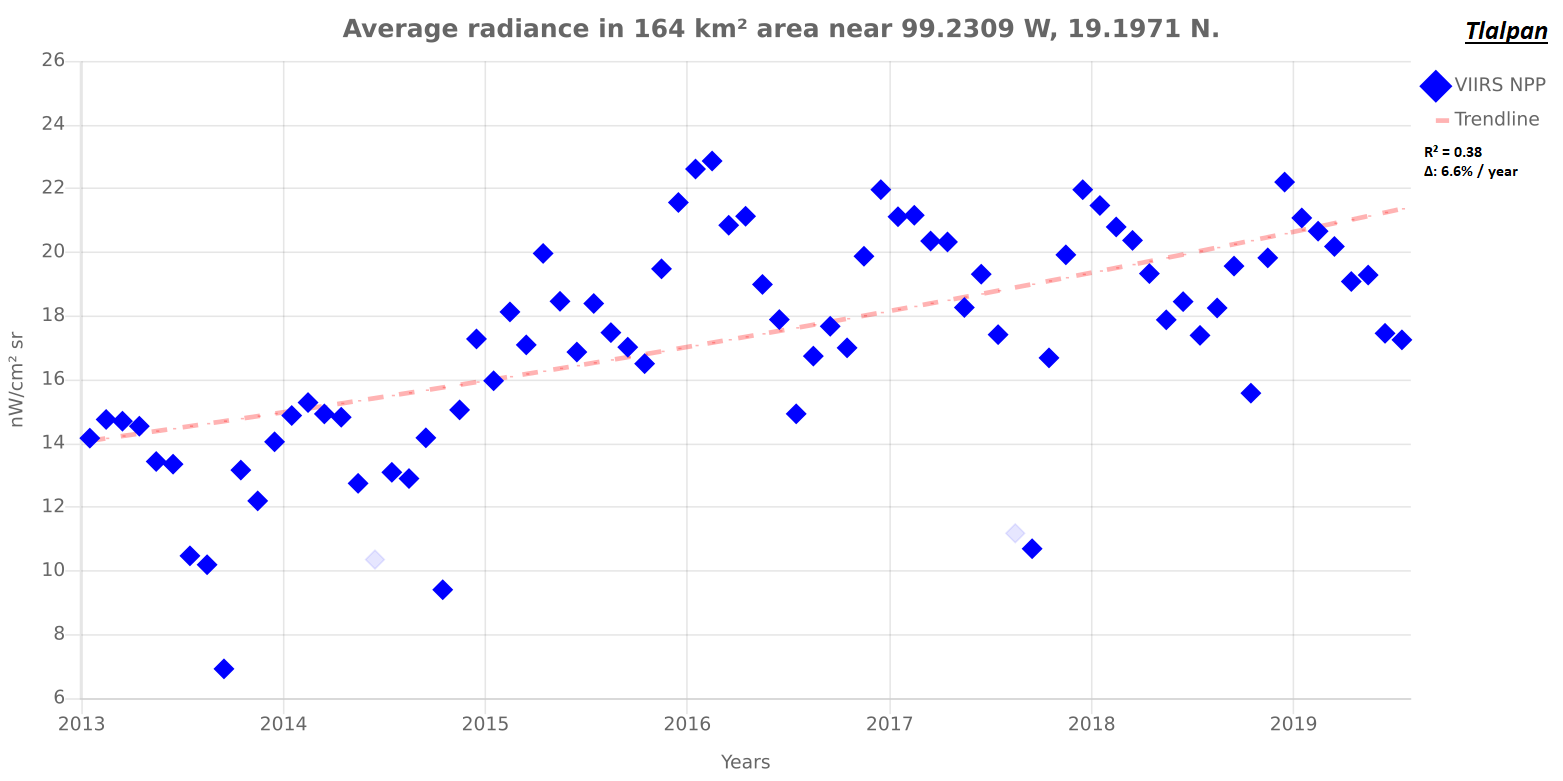
\includegraphics[width=1\textwidth]{TLA}
  \caption{Tendencia de radiancia promedio para la alcaldía Tlalpan}
  \label{radiancetrendstla}
\end{figure}
\blindtext

\newpage

\begin{figure}[H]
  \centering
    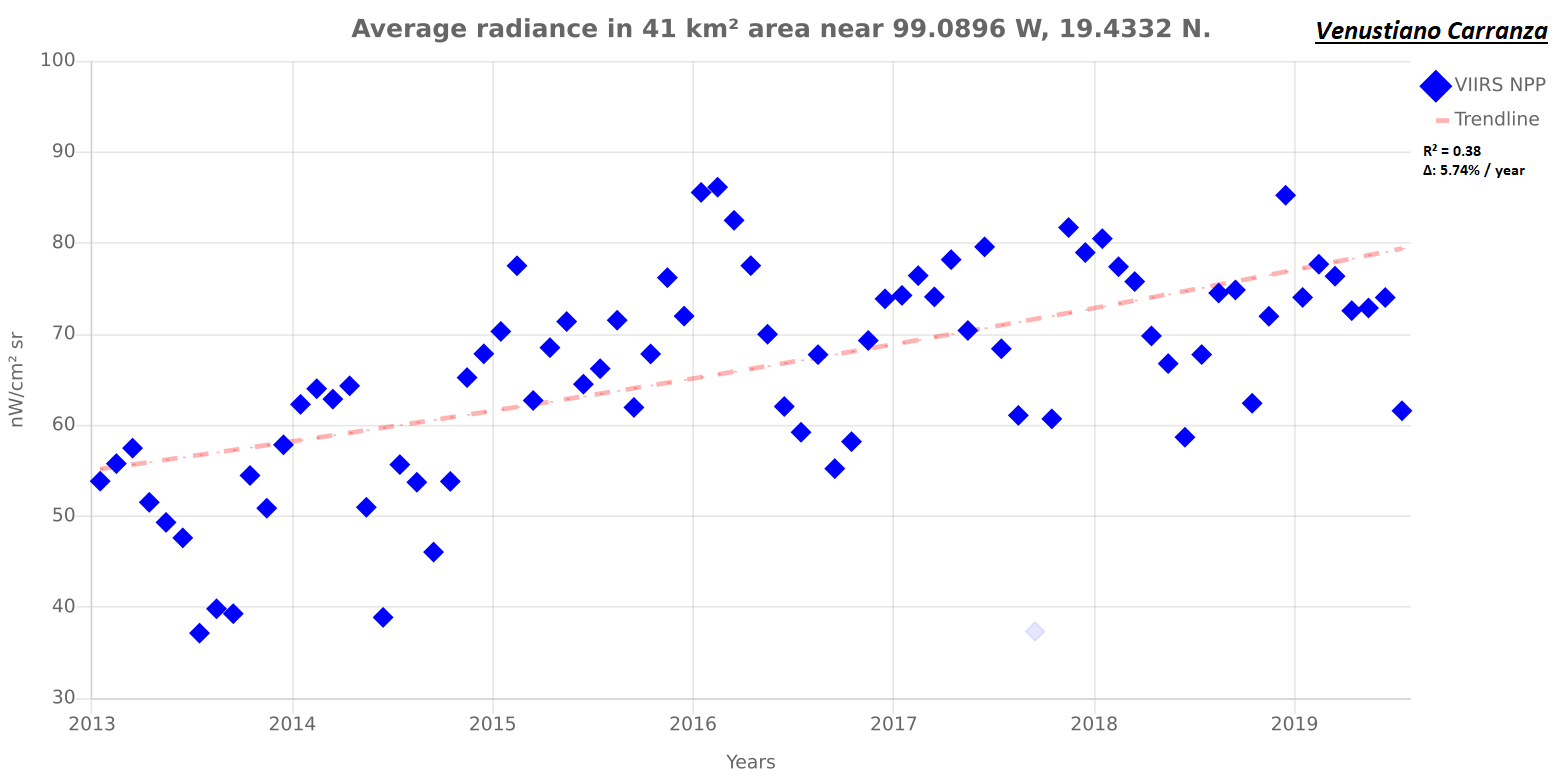
\includegraphics[width=1\textwidth]{VC}
  \caption{Tendencia de radiancia promedio para la alcaldía Venustiano Carranza}
  \label{radiancetrendstlah}
\vspace{20mm} 
    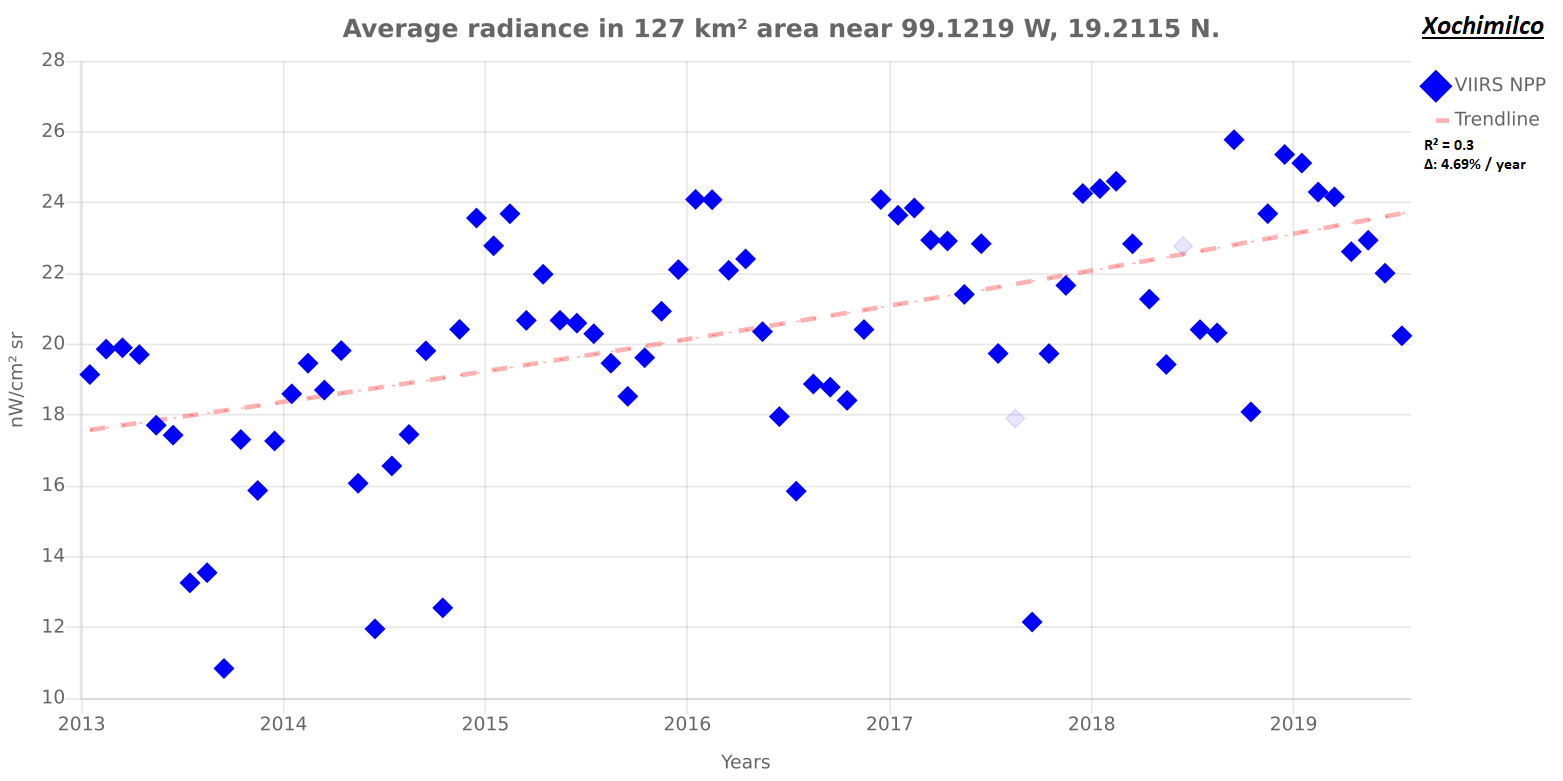
\includegraphics[width=1\textwidth]{XO}
  \caption{Tendencia de radiancia promedio para la alcaldía Xochimilco}
  \label{radiancetrendstla}
\end{figure}
\blindtext

\newpage